\section{Methods} \label{sec:methods}

Three independent experiments were performed to test alternate inference techniques over sexual populations: genealogical inference, effective population size inference, and positive selection inference.

Section \ref{sec:instrumentation} reviews hereditary stratigraphic annotation methodology as originally developed for inference over asexual populations and introduces the gene- and species-level instrumentation strategies proposed to apply it to sexual populations.
The former strategy is used for positive selection inference and the later is used for genealogical and population size inference.

Section \ref{sec:gene-drive} overviews the recombination and gene drive mechanisms employed for species-level instrumentation.
Section \label{sec:collision-probability} evaluates the extent to which this methodology increases the expected rate of spurious differentia collision, which can lead to overestimation of relatedness from hereditary stratigraph instrumentation.

Section \ref{sec:one-max} describes the toy ``one-max'' problem used for the genealogical inference and population size inference experiments.

Section \ref{sec:genealogical-inference} describes the three treatments compared to test the proposed genealogical inference mechanisms.
Section \ref{sec:phylogeny-extraction} lays details the procedure used to convert recorded sexual pedigrees to phylogenetic trees that reconstruction quality could be evaluated against.

Section \ref{sec:population-size-inference-principle} recaps the mechanistic principle behind distributed population size estimation and Section \ref{sec:population-size-inference-stats} reports statistical formulations derived to perform distributed population size estimation.
Section \ref{sec:ne-process-example} explains population size inference over an example evolutionary replicate.

Section \ref{sec:population-size-inference-experiments} describes the three treatments compared to test the proposed population size inference mechanism.

Section \ref{sec:dist-gene-prevalence-est} summarizes the proposed mechanism for gene selection inference and Section \ref{sec:positive-selection-inference-experiment} reports the evolutionary system and experimental treatments used to test it.

Finally, Section \ref{sec:software-data} acknowledges open source software used in this work and links to software and other artifacts from the work.

\subsection{Hereditary Stratigraphy Instrumentation}
\label{sec:instrumentation}

\begin{figure}
  \centering
  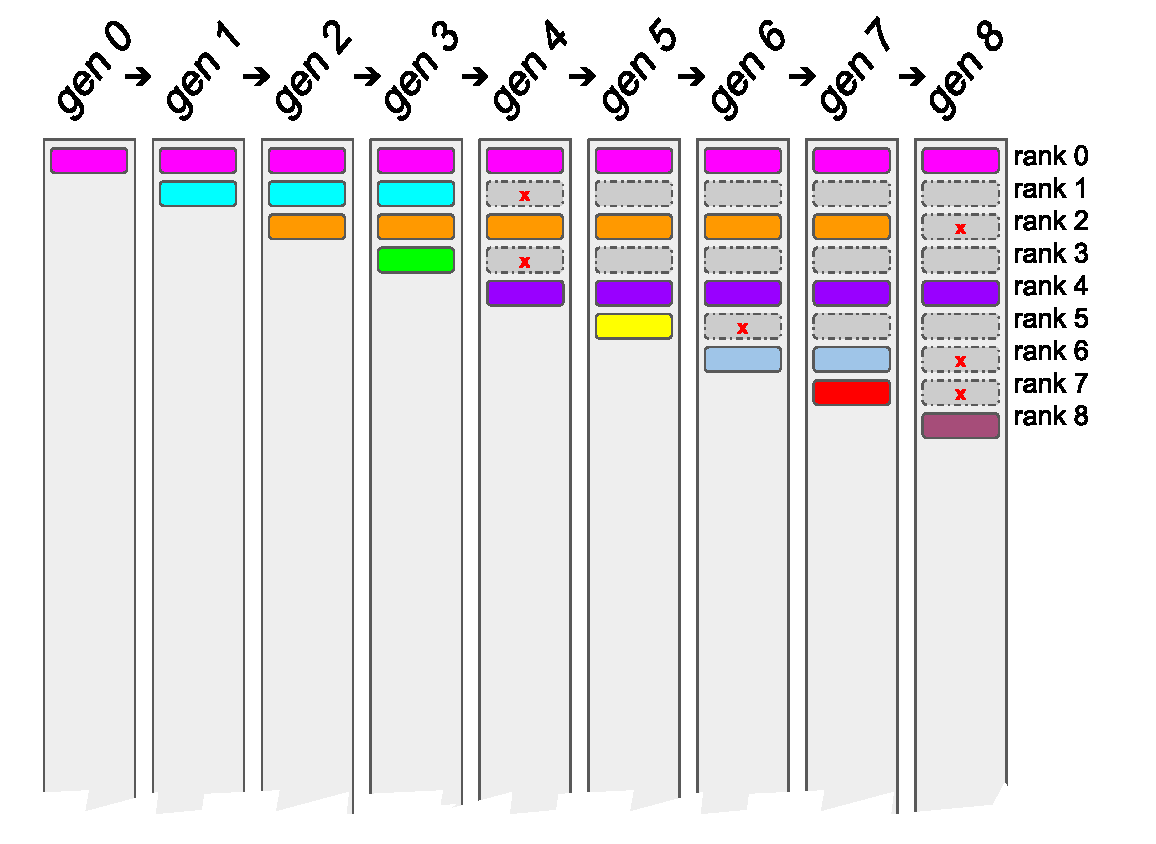
\includegraphics[width=\textwidth]{img/deposit-prune-example}
  \caption{
    TODO
  }
  \label{fig:deposit-prune-example}
\end{figure}

\begin{figure}
  \centering
  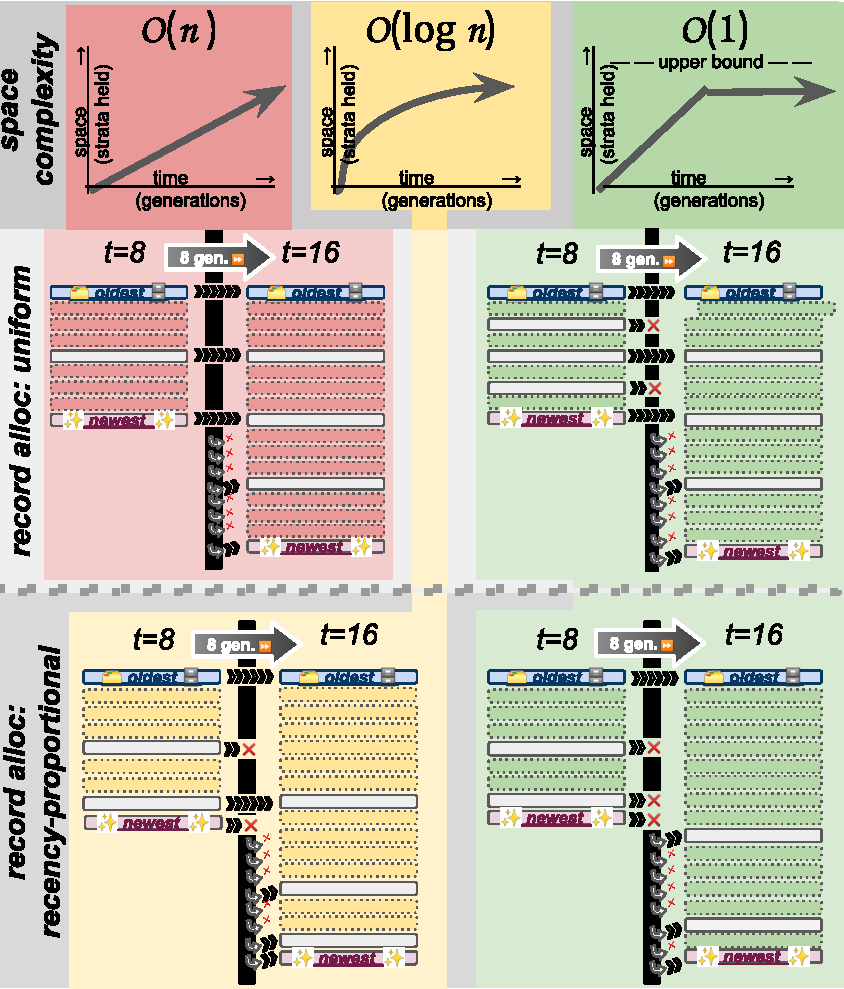
\includegraphics[width=\textwidth]{img/retention-policy-matrix}
  \caption{
    Comparison of four stratum retention policies by space complexity per stratigraph with respect to generations elapsed (columns, red/yellow/green) and by distribution of retained differentia (rows).
    Uniform allocation keeps differentia in evenly-spaced layers.
    Recency-proportional allocation keeps more more-recent differentia, trading off coarser resolution to infer ancient phylogenetic events for finer resolution to infer recent phylogenetic events.
    Retained layers under each policy are shown at $t=8$ generations and $t=16$ generations, with new differentia being deposited in a descending fashion.
    Differentia pruning events are noted with a red $x$.
  }
  \label{fig:retention-policy-matrix}
\end{figure}


Proposed methods for genealogical and evolutionary inference over distributed sexual populations build on the recently-developed ``hereditary stratigraphy'' technique, originally developed to facilitate phylogenetic inference over asexual populations \citep{moreno2022hstrat}.
This approach applies heritable markers to individual digital genomes to facilitate post-hoc reconstruction of phylogenetic history.
Each time a marker is inherited, a fresh random packet of data --- a ``fingerprint'' --- is generated and appended to the inherited marker.
To infer phylogenetic history, fingerprints from the markers of extant organisms are aligned and compared.
Identical fingerprints within the record signifies (likely) shared ancestry between organisms.
Conversely, the presence of a discrepancy in fingerprints definitively evidences divergence in ancestry at the generation those fingerprints were generated.

Without additional mechanisms, genome marker size would grow linearly as generations elapse and quickly become unwieldy.
Abatement of such instrumentation bloat necessitated development of a library of strategies for on-line pruning of fingerprints within markers.
Discarding fingerprints decreases annotation size at the cost of sparsifying time points at which  ancestral similarity or differentiation is observable.
Trade-offs between annotation size and estimation accuracy can therefore be tuned through fingerprint retention strategy.
For instance, resolution may be maintained over time points as a fixed proportion of generations elapsed since those time points at the cost of logarithmic growth in annotation size.
Or, another possibility, annotation size can be maintained below a constant bound at the cost of linear growth in uncertainty as generations elapse.

Fingerprint pruning was not performed in the reported experiments in order to simplify experimental setup and analysis.
This means that a complete annotation record with fingerprints corresponding to every generation was maintained.
Population-size and gene-selection inference mechanisms introduced here are in principle compatible with fingerprint pruning.
Effective application of hereditary stratigraphy to sexual populations in practice, will require further work to determine the most effective distribution of fingerprint retention (e.g., uniform across generational time versus recency-proportional favoring more recent events) and the levels of reconstruction accuracy pertinent to characterization of evolutionary history and dynamics \citep{moreno2023toward}.

This work uses 64 bit fingerprints, which collide with probability $1/2^{64} \approx 5 \times 10^{-20}$.
At population size 100 over 200 generations, as in the genealogical inference and control condition of the population size inference experiments, the probability of any collision is $< 2 \times 10^{-15}$.
At population size 200 over 400 generations, as in the gene selection inference experiments, the probability of any collision is $< 5 \times 10^{-15}$.

\begin{SCfigure}[3][b]
  \centering
  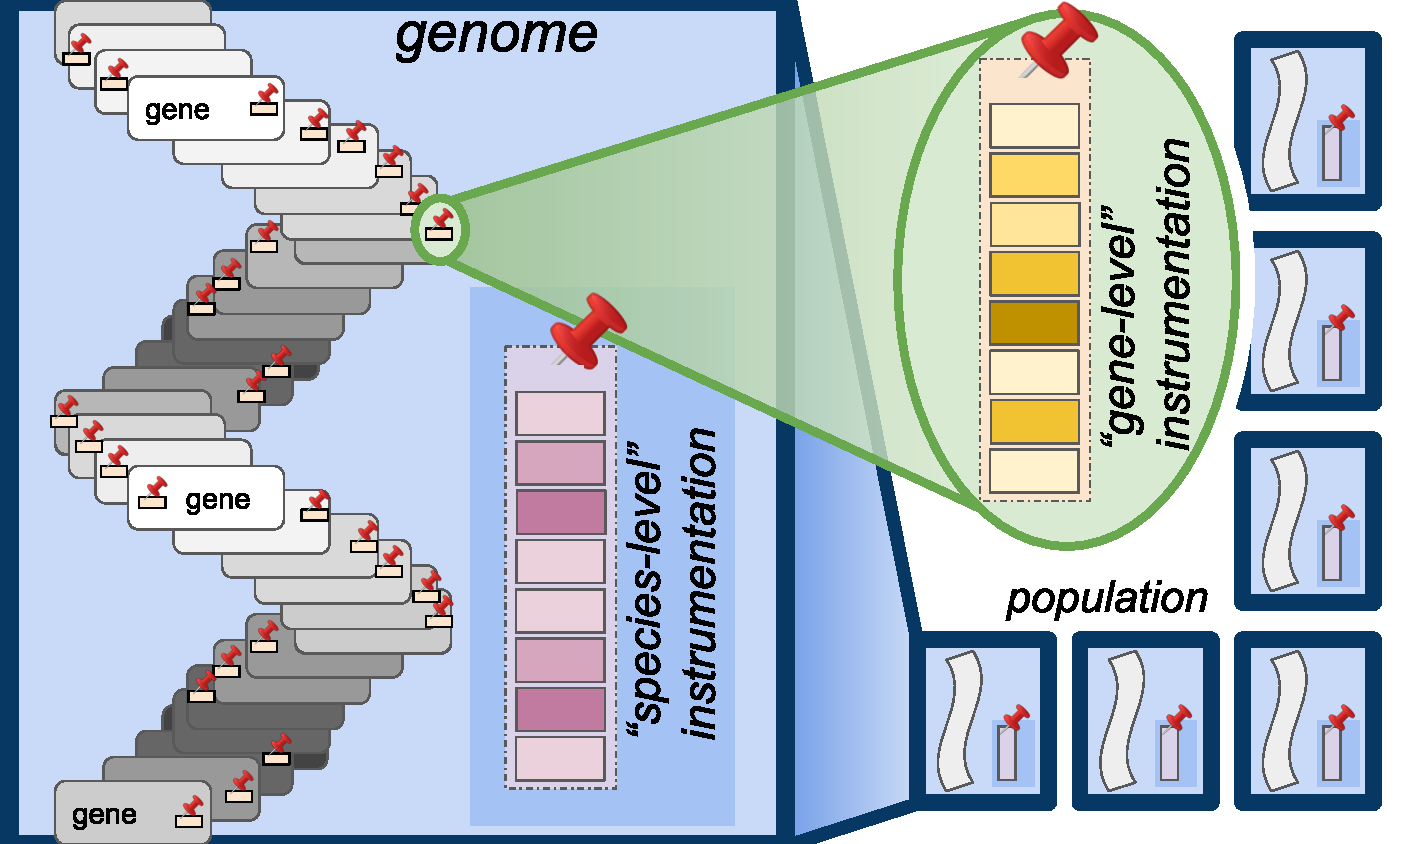
\includegraphics[width=0.5\textwidth]{img/annotation-types}
  \caption{
    Proposed instrumentation methods: ``species-level'' and ``gene-level'' instrumentation.
    Each organism has a single hereditary stratigraph attached as species-level instrumentation, with a gene drive mechanism (Figure \ref{fig:gene-drive}) ensuring consistentcy within species (i.e., interbreeding populations).
    Gene-level instrumentation associates instrumentation with individual genes, to be used for gene tree reconstructions.
  }
  \label{fig:annotation-types}
\end{SCfigure}


As originally devised for asexual populations, hereditary stratigraphic markers followed a one-to-one relationship to genomes.
Here, we explore two alternate schemes designed for instrumentation of sexual populations: gene instrumentation and species instrumentation.

The former treats individual genes as asexual subcomponents of sexual lineages, instrumenting genes individually using the original hereditary stratigraphy methodology.
This strategy involves (potentially) several independent hereditary stratigraph instruments per organism.
In, along the lines of ``gene tree'' analsyes in traditional phylogenetics \citep{avise1989gene}.

In cases where digital chromosomes comprise a relatively small number of atomic genes, it may make sense to instrument every gene independently.
However, in applications with very fine atomic genes (e.g., individual GP instructions) or no atomic genes (e.g., GA floating point values subjected to interpolation during crossover) it may make sense to instrument a representative subset of genes or introduce ``dummy'' genes associated with certain chromosomal positions.

Species-level instrumentation operates via hereditary stratigraphic columns associated with individual genomes.
Instrumentation consensus within interbreeding populations is achieved through a gene drive mechanism that forces a single consensus differentia value to sweep each hereditary stratigraph layer (described in Section \ref{sec:gene-drive}).
Although gene drive mechanisms are widespread in natural systems \citep{alphey2020standardizing, price2020resistance}, unlike gene-level annotation this technique has no direct analogy in typical phylogenetic analyses.

Species instrumentation employed the recombination and gene drive mechanism described in Section \ref{sec:gene-drive}.
Species hereditary stratigraph instrumentation was employed for the genealogical inference and population size inference experiments.
Gene instrumentation employed the distributed copy count estimation mechanism described in Section \ref{sec:dist-gene-prevalence-est}.
Gene hereditary stratigraph instrumentation was employed for the positive selection inference experiment.

\subsection{Hereditary Stratigraphic Column Recombination \& Gene-drive Mechanism}
\label{sec:gene-drive}

\begin{SCfigure}[3][b]
  \centering
  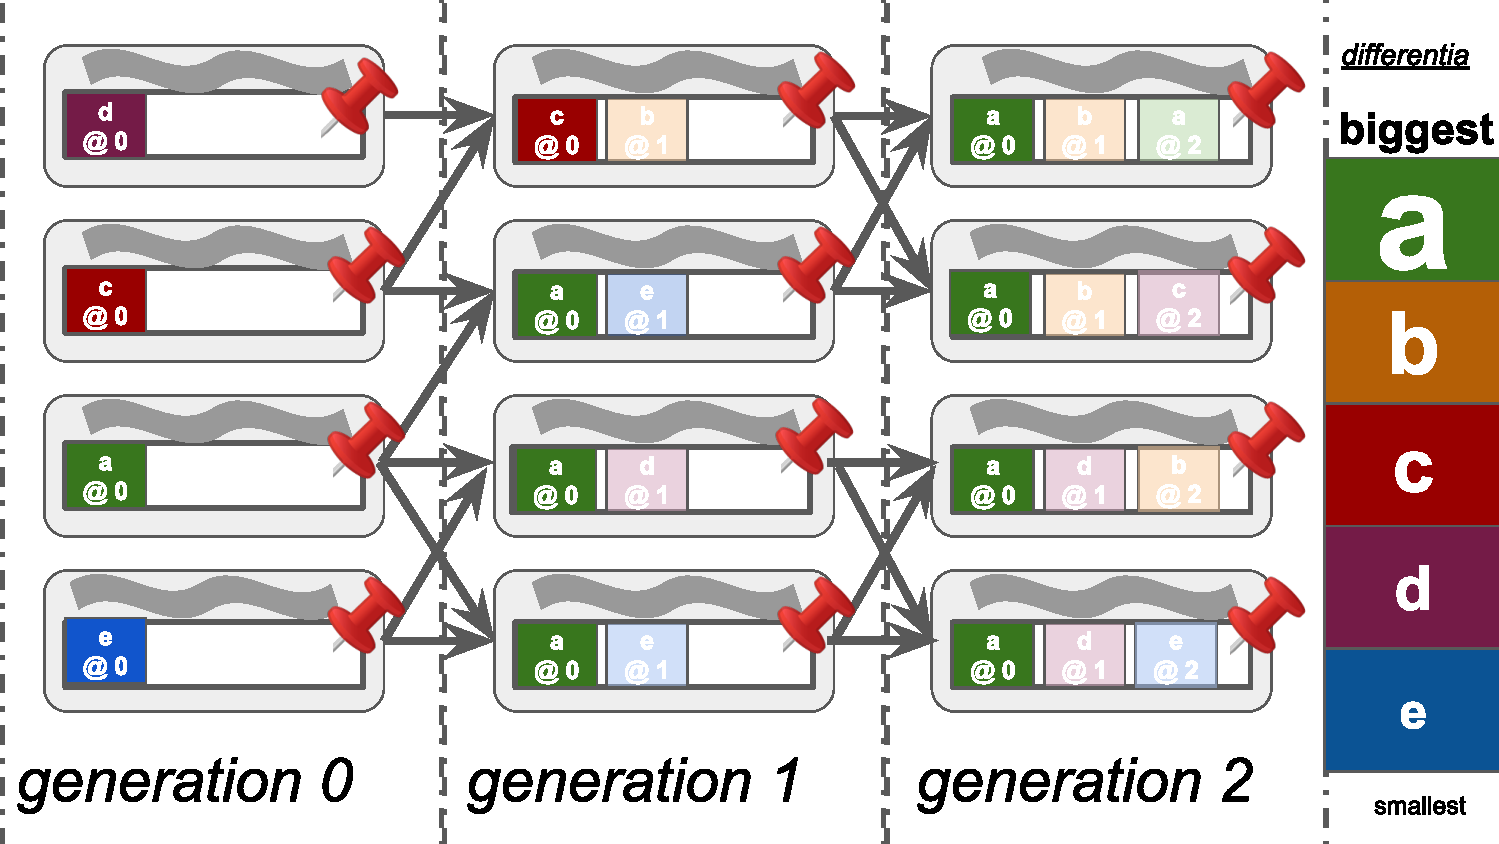
\includegraphics[width=0.6\textwidth]{img/gene-drive}
  \caption{
    Gene drive mechanism for species-level instrumentation.
    The larger of parents' differentia values at each layer is inherited.
    The largest value generated among layer 0 differentia ($a$) spreads from one member at generation 0 to all four by generation 2.
    This mechanism applies to ``species-level'' instrumentation (Figure \ref{fig:annotation-types}).
  }
  \label{fig:gene-drive}
\end{SCfigure}


Successful species-level tracking necessitates consistent labeling of interbreeding population members and consensus among members on phylogenetic history.
In the hereditary stratigraphic context, this translates to consistency in ``fingerpint'' differentia values for each instrumentation layer among population members.
Recombination of differentia values between genome instrumentaiton markers will, in the limit, enforce such consensus.
Under such a scheme, offspring would inherit differnetia values at each instrumentation layer independently, with values assigned to the offspring's instrumentation layers chosen arbitrarily from the corresponding layer of either of the parents.
As $t \to \infty$, a single consensus fingerprint will eventually fix at each instrumentation layer within the population through drift.
However, expected time to coalescence can be long for large populations.
Further, distributions of coalescence times is fat-tailed, meaning that time for \textit{all} sites to reach consensus would be prohibitively large in most cases.

A simple inheritance rule induces faster consensus: the larger of parents' differentia values at each instrumentation layer is inherited by all offspring.
In well-mixed populations and structured populations with long-distance migration, copy count of the largest-magnitude differentia value will grow more or less exponentially until reaching fixation (making time-to-fixation a logarithmic function of population size).

Asynchronous generations slightly complicate the picture.
When individuals from different generations recombine, one parent will necessarily have instrumentation layers not present in the other.
How should recombination proceed in this case?
One possibility would be to simply ``fast-forward'' the younger instrument to match the generational depth of the elder.
As with fingerprint pruning, species-level geneaology and population size inference mechanisms introduced here are in principle compatible with crossover between hereditary stratigraph instrumentation with mismatched generations.
Synchronous generations were used for experiments reported in this work, however, so full exploration of this consideration remains for future work.

The described recombination and gene drive mechanism only applied to species-level instrumentation and was used for the genealogical and population size inference experiments.

\subsection{Collision Probability Between Fixed Differentia Genes}
\label{sec:collision-probability}

Fixed genes' skew toward large-magnitude integers due to the dominance of larger values in gene drive competition increases the probability of fixed-gene collision between two populations causing misdetection of shared ancestry between the populations.
Quantifying this collision probability effect is key to predicting the efficacy of this approach at scale.

Suppose independent populations of size $a$ and $b$.
The largest gene in each population will drive to fixation.
If each population members' gene is drawn from uniform distribution on integers $[0, u)$, then the probability of collision between the populations' fixed genes is

\begin{align*}
\frac{a \sum_{n=1}^{a + b - 1} \frac{u^{- n - 1} \left(\frac{u - 1}{u}\right)^{a + b - n - 1} \left(- \frac{{\binom{a - 1}{n}}}{{\binom{a + b - 1}{n}}} + 1\right) {\binom{a + b}{n + 1}}}{1 - \left(\frac{u - 1}{u}\right)^{a + b - 1}}}{a + b} \\
+ \frac{b \sum_{n=1}^{a + b - 1} \frac{u^{- n - 1} \left(\frac{u - 1}{u}\right)^{a + b - n - 1} \left(- \frac{{\binom{b - 1}{n}}}{{\binom{a + b - 1}{n}}} + 1\right) {\binom{a + b}{n + 1}}}{1 - \left(\frac{u - 1}{u}\right)^{a + b - 1}}}{a + b}.
\end{align*}

Derivation will be provided in supplementary materials.

For 32-bit differentia $u = 2^{32}$, collision occurs with $p < 0.5$ for two populations of size $a = b = 2 \times 2^{31}$ .
Collision occurs with $p < 0.01$ for two populations of size $a = b = 2^{26}$.
So, for 32-bit differentia populations with magnitude below a factor of 64 of the maximum representable differentia value, collision probability between is low.
Numerical considerations complicate evaluation of similar results for $u = 2^{64}$.

\subsection{One-Max Task}
\label{sec:one-max}

We used the one-max task for experiments to evaluate population size inference and genealogical inference.
This tasks selects over fixed-length bit string individuals for the fraction of 1's set.
Each individual was represented as a binary string of length 100.
Fitness was evaluated as the sum of the bits in the binary string, preferring individuals with more 1s over individuals with fewer.
Population size was 200 individuals, initialized randomly with sites set to 1 with probability 0.5.
In treatments where population size decreased during an evolutionary run, excess individuals were eliminated randomly.
In treatments where population size increased during an evolutionary run,
new population slots were filled through selection over the existing population.

Selection was performed using the tournament selection method.
Default tournament size was 2.
Tournament sizes 1 and 8 were also set in some treatments.
Tournaments were performed synchronously, with all parents selected before turnover of the entire population.
Evolutionary runs lasted 100 generations.

Two-point crossover (mating) and bit-flip mutation with per-bit probability 0.05 were applied to all organisms at all generations prior to selection.

Operator choice and parameter selections were based on one-max example code from the Distributed Evolutionary Algorithms in Python package \citep{fortin2012deap}.

\subsection{Genealogical Inference Experiment}
\label{sec:genealogical-inference}

This experiment tested the quality of genealogical history recovered from species-level hereditary stratigraph annotation.
Phylogenetic reconstruction quality was tested over three evolutionary treatments.
The first, ``allopatry,'' covered full speciation through introduction of a strict reproductive barrier among subpopulations.
The second, ``ring,'' covered partial phylogenetic structure over subpopulations linked through small amounts of migration.
A third --- as a control --- was designed to lack meaningful phylogenetic structure at all due to well-mixed interbreeding ensuring close relatedness between all population members.
Ten independent replicates were performed for each treatment.

The experiment was performed on the one-max problem domain described in Section \ref{sec:one-max}.
After the 200th and final generation, the species-level annotations extracted from each of the extant organisms.
Phylogenetic structure was reconstructed using from these annotations using the agglomerative trie-based reconstruction techniques developed in \citep{moreno2023toward}.
(Essentially, the phylogeny is constructed so that organisms track the lineage they share the most consecutive ``fingerprint'' differentia with and then branch out at the point of the first disparity in differentia value.

To evaluate reconstruction quality, inferred phylogenies were compared to references extracted directly from underlying sexual pedigree record of the simulation using the MRCA-based UPGMA methods described in Section \ref{sec:phylogeny-extraction}.
Disagreement between reconstruction and reference was quantified using the quartet tree distance metric \citep{estabrook1985comparison}.

Additionally, inferred phylogenies were visualized to confirm whether reconstructions recovered the major features of treatments' evolutionary histories.

\subsubsection{Allopatry Treatment}

This treatment simulates 100 generations of well-mixed sympatric evolution.
At generation 100, the population is divided into two 50-member subpopulations.
These subpopulations evolve independently with no migration for 50 generations.
Then, at generation 150, the first subpopulation is split again into .
The remaining 50-member subpopulation and the five new 10-member subpopulations then evolve independently with no migration for a further 50 generations.
Phylogenetic reconstruction from this treatment should ideally recover a binary branching at generation 100 followed by a secondary quintuple-branching along one lineage at generation 150.

\subsubsection{Ring Treatment}

This treatment splits the population into ten distinct subpopulations (islands), each of which evolved independently.
The subpopulations were arranged in a ring topology, and one individual migrated between adjacent populations per generation happens once per generation.

\subsubsection{Bag Treatment}

This treatment selects and recombines individuals uniformly from across the entire population.
As such, all individuals extant at simulation completion are closely related so no meaningful phylogenetic structure exists to be detected.

\subsection{Phylogeny Extraction from Pedigree Records}
\label{sec:phylogeny-extraction}

In order to provide a baseline reference to evaluate annotation-based phylogenetic reconstructions against, phylogenetic relationships between extant organisms (i.e., an asexual tree describing ``relatedness'') were extracted from sexual pedigrees (i.e., a reticulated directed acyclic graph describing ancestry).

Such conversion has fundamental limitations: in well-mixed populations of modest size, structured differences in phylogenetic relatedness do not meaningfully exist.
However, speciation and spatial structure can introduce meaningful aspects of phylogenetic structure.

A naive technique was used to distill phylogenetic relationships from pedigree data.
Most Recent Common Ancestors (MRCA) were computed pairwise from the pedigree data to construct a distance matrix among extant individuals.
Unweighted Pair Group Method with Arithmetic mean (UPGMA) reconstruction based on this distance matrix yielded inferred phylogenetic structure \citep{sokal1958university}.
Finally, corrections to branch lengths were performed to accurately position the terminal nodes (i.e., extant organisms) at their known generational depths.

No effort was made to cluster extant organisms into taxa based on a relatedness threshold, so reconstructions contained non-informative branch structure among closely-related individuals.

\subsection{Population Size Inference Principle}
\label{sec:population-size-inference-principle}

Consider a population composed of $n$ individuals, each holding a unique gene represented as an unsigned integer of a given precision.
At the outset, each gene value is assumed to be drawn from a uniform distribution across all possible values.
As generations evolve through sexual recombination, a "gene drive" mechanism is enforced where offspring inherit the larger gene value from their parents.
Over time, this mechanism results in the largest gene value becoming dominant or `fixed' in the population.

An interesting property of this gene drive mechanism is the potential to estimate the original population size by observing the distribution of the fixed gene values.
By introducing a random variable $\mathbb{X}$ to represent the magnitude of the fixed gene value, we can explore its distribution. Assuming our gene value is uniformly distributed between 0 and 1, it is identified as $\beta(n, 1)$ \citep{gentle2009computational} distributed.
Hence, by observing the values of these fixed genes, it's possible to infer $n$, the original population size.
This approach is further extendable to cases involving multiple independent genes, each adhering to the same fixed precision and initial uniform distribution, providing a compelling estimation technique for population size.

Directly analogous techniques to estimate population size have also arisen in the context of decentralized, anonymous network engineering \citep{varagnolo2010distributed,hakan2012distributed}.
In these schemes, nodes independently draw a random vector of numerical values from a known distribution.
Values are exchanged through an aggregating function like (e.g., minimum, maximum, etc.), ultimately resulting in a consensus value fixing within the network.
Each node can then independently infer probabilistic information about the larger network, in a manner that is generally consistent across nodes.

\subsection{Population Size Inference Statistics}
\label{sec:population-size-inference-stats}

Statistical details necessary to work with the fixed-gene-magnitude inference method follow, some of which are, to best knowledge, not yet reported.
Derivations are available at \url{https://github.com/mmore500/hereditary-stratigraph-concept/tree/master/binder/popsize}, and will be included in supplemental material.

\subsubsection{Maximum Likelihood Estimator}

The maximum likelihood estimator for population size given $i$ independent observations of fixed-gene magnitude $x_i$ is
\begin{align} \label{eqn:popsize_mle}
\hat{n}_\mathrm{mle} = -\frac{k}{\sum_{i=1}^k \log( x_i )}.
\end{align}

This estimator was also derived in \citep{varagnolo2010distributed}.

\subsubsection{Maximum Likelihood Estimator Mean Square Error}

Mean square error of the maximum likelihood estimator for population size given $k$ observations of fixed gene magnitude is

\begin{align*}
n^2 \frac{k^{2}+ k-2}{(k-1)^{2}(k-2)}.
\end{align*}

This result was also derived in \citep{varagnolo2010distributed}.

\subsubsection{Maximum Likelihood Estimator Expected Value}

Expected value for the maximum likelihood population size estimator $\hat{n}_\mathrm{mle}$ is given as

\begin{align*}
E(\hat{n}_\mathrm{mle})
= n\frac{k}{k-1}
\end{align*}

for $k>1$ \citep{varagnolo2010distributed}.
This value can be subtracted from the maximum likelihood estimator to yield a mean-unbiased population size estimator.

\subsubsection{Confidence Interval}

Computation of confidence intervals is necessary of facilitate experimental inference from population size estimators.
Formulations derived from the maximum likelihood estimator are provided below.

For a single observation of fixed gene magnitude $\hat{x}$, the population size $n$ can be estimated with $c\%$ confidence to fall within the interval

\begin{align*}
\Big(
\frac{\log(\frac{1+c/100}{2})}{\log\hat{x}},
\frac{\log(\frac{1-c/100}{2})}{\log\hat{x}}
\Big).
\end{align*}

The 95\% confidence interval spans a 145-fold order of magnitude and a 99\% confidence interval spans a 1057-fold order of magnitude.

For $k$ observations of fixed gene magnitude $\hat{x}_i$, the population size $n$ can be estimated with $c\%$ confidence to fall within the interval $(\hat{n}_\mathrm{lb}, \hat{n}_\mathrm{ub})$ where $\hat{n}_\mathrm{lb}$ is the solution to

\begin{align} \label{eqn:popsize_mle_ci_lb}
0
&= 2\Gamma(k, -\hat{n}_\mathrm{lb}\log(\prod_{i=1}^k\hat{x}_i)) - (c/100+1)\Gamma(k)
\end{align}

and $\hat{n}_\mathrm{ub}$ is the solution to

\begin{align} \label{eqn:popsize_mle_ci_ub}
  0
  &= 2\Gamma(k, -\hat{n}_\mathrm{ub}\log(\prod_{i=1}^k\hat{x}_i))) - \Gamma(k)(1-c/100).
\end{align}

Four independent observations are sufficient to provide a 95\% confidence interval spanning 8-fold magnitude or a 99\% confidence interval spanning a 16-fold magnitude.
Nine independent observations are sufficient for a 95\% confidence interval spanning a factor spanning 4-fold magnitude or a 99\% confidence interval spanning a factor of 6-fold magnitude.
33 independent observations are sufficient for a 95\% confidence interval spanning 2-fold magnitude or a 99\% confidence interval spanning 2.5-fold magnitude.

Note that the width of the confidence interval will scale as a constant factor of as $n \to \infty$.

\subsubsection{Median-unbiased Estimator}

A median-unbiased estimator $\hat{n}_\mathrm{mle}$ for population can be trivially derived from the confidence interval, as the numerical solution of

\begin{align*}
0
&= 2\Gamma(k, -\hat{n}_\mathrm{mumle}\log(\prod_{i=1}^k x_i)) - \Gamma(k).
\end{align*}

\subsubsection{Credible Intervals}

Computation of credible intervals facilitates bayesian experimental inference from population size estimators.
Derivation assumes a uniform prior over population size.
The credibility contained within a factor of the maximum likelihood estimate $\hat{n}_\mathrm{mle}$ can be calculated as


\begin{align*}
\frac{- \gamma(k + 1, \frac{k}{f}) + \gamma(k + 1, f k)}{k!}.
\end{align*}

By its form, the credibility contained within a factor of maximum likelihood estimate remains constant across population sizes $n$.
Credibility intervals require similar sample sizes to provide $n$-fold magnitude spans as those for confidence intervals discussed above.

\subsubsection{Rolling Population Size Estimation} \label{sec:rolling_estimation}

Experiments reported here use a simple rolling process to aggregate ten preceding fixed-gene magnitudes to compute a population size estimate and confidence intervals.
More sophisticated regularizations have been proposed to consolidate time series estimates of dynamically-changing network sizes \citep{hakan2012distributed}.

\subsection{Example Population Size Inference}
\label{sec:ne-process-example}

\begin{figure}
  \centering

  \begin{minipage}{.65\textwidth}
    \centering
    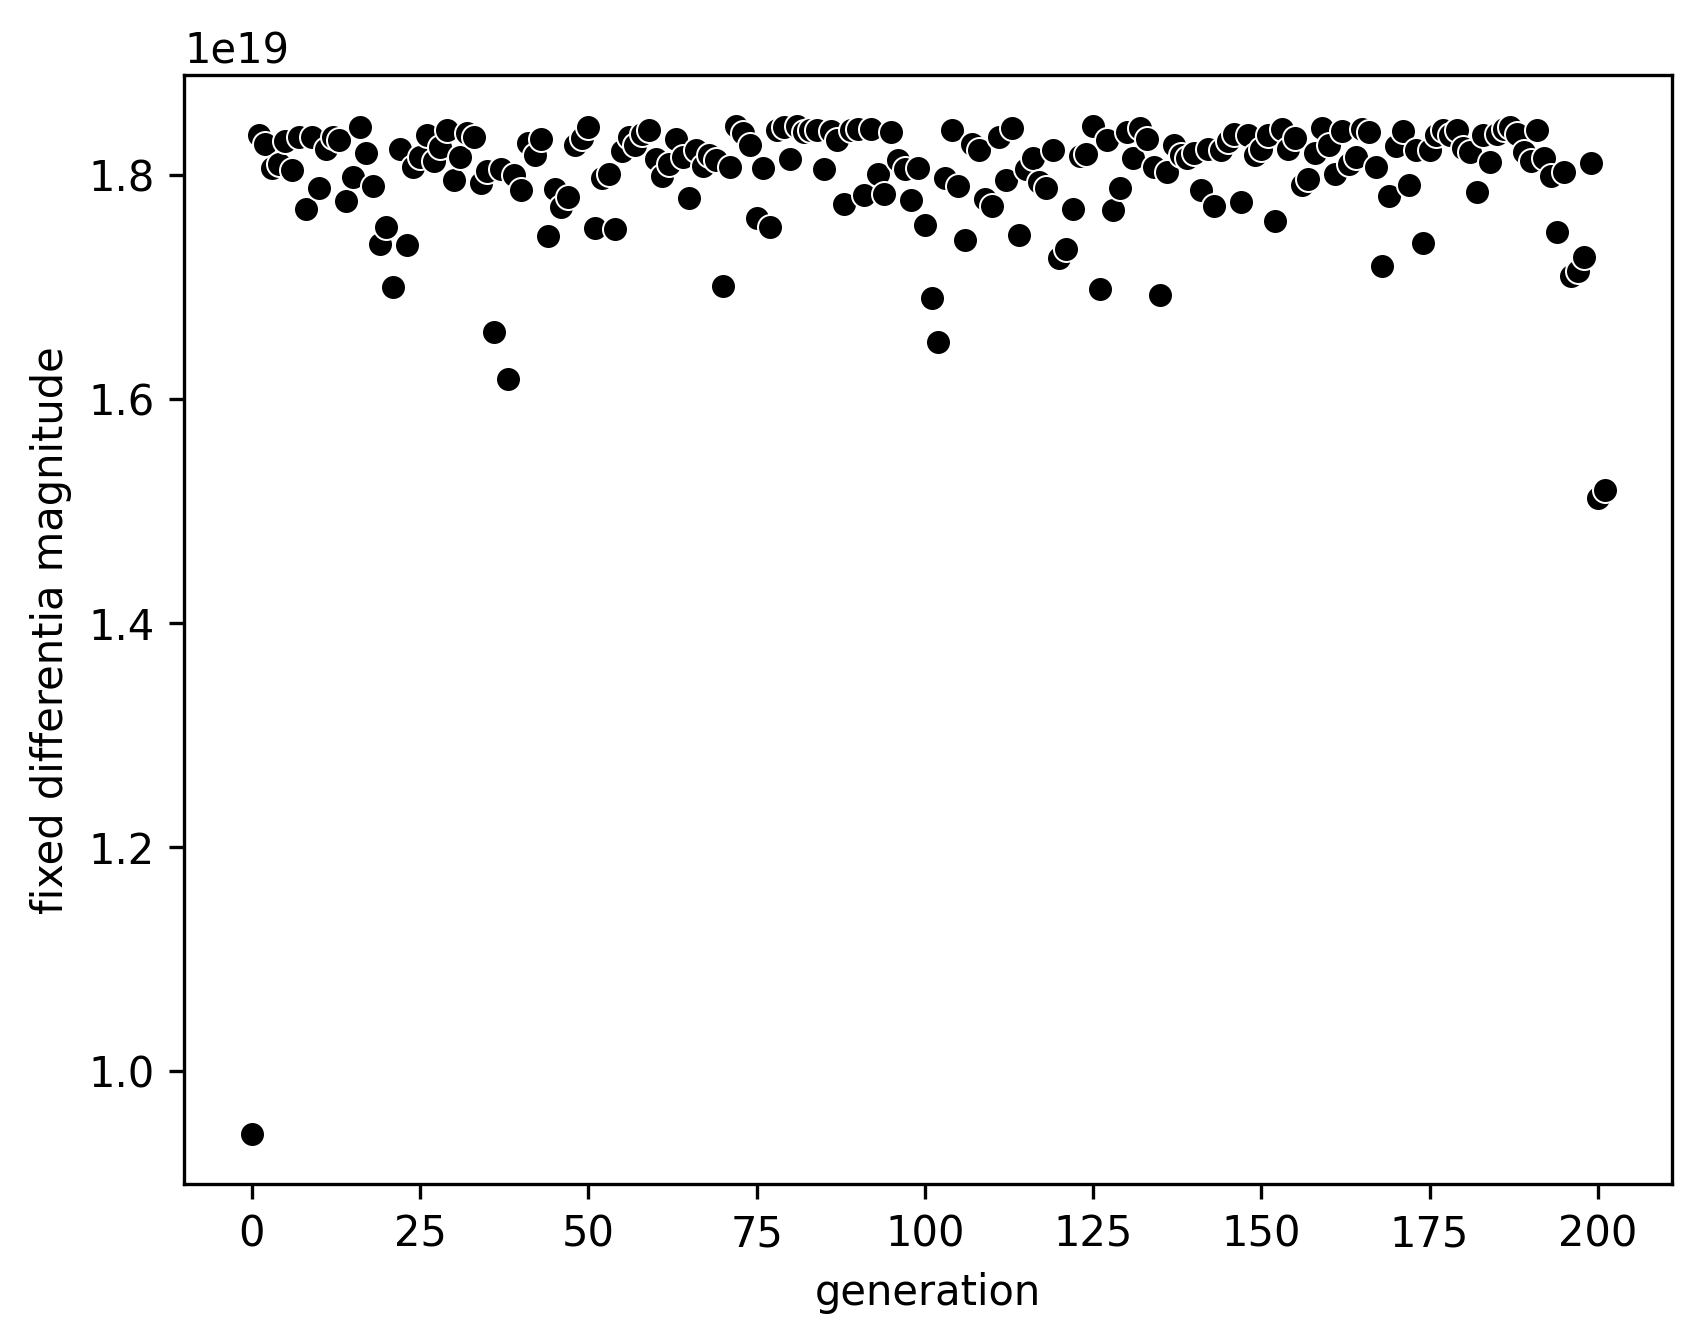
\includegraphics[height=0.25\textheight]{notebooks/notebooks/teeplots/notebook=ne-inference+replicate=0+treatment=control+viz=scatterplot-differentia-magnitude+ext=}
  \end{minipage}%
  \begin{minipage}{.25\textwidth}
    \subcaption{Fixed Species-level Differentia Magnitudes by Layer}
    \label{fig:ne-process-example:differentia}
  \end{minipage}

  \vspace{0.25em}

  \begin{minipage}{.65\textwidth}
    \centering
    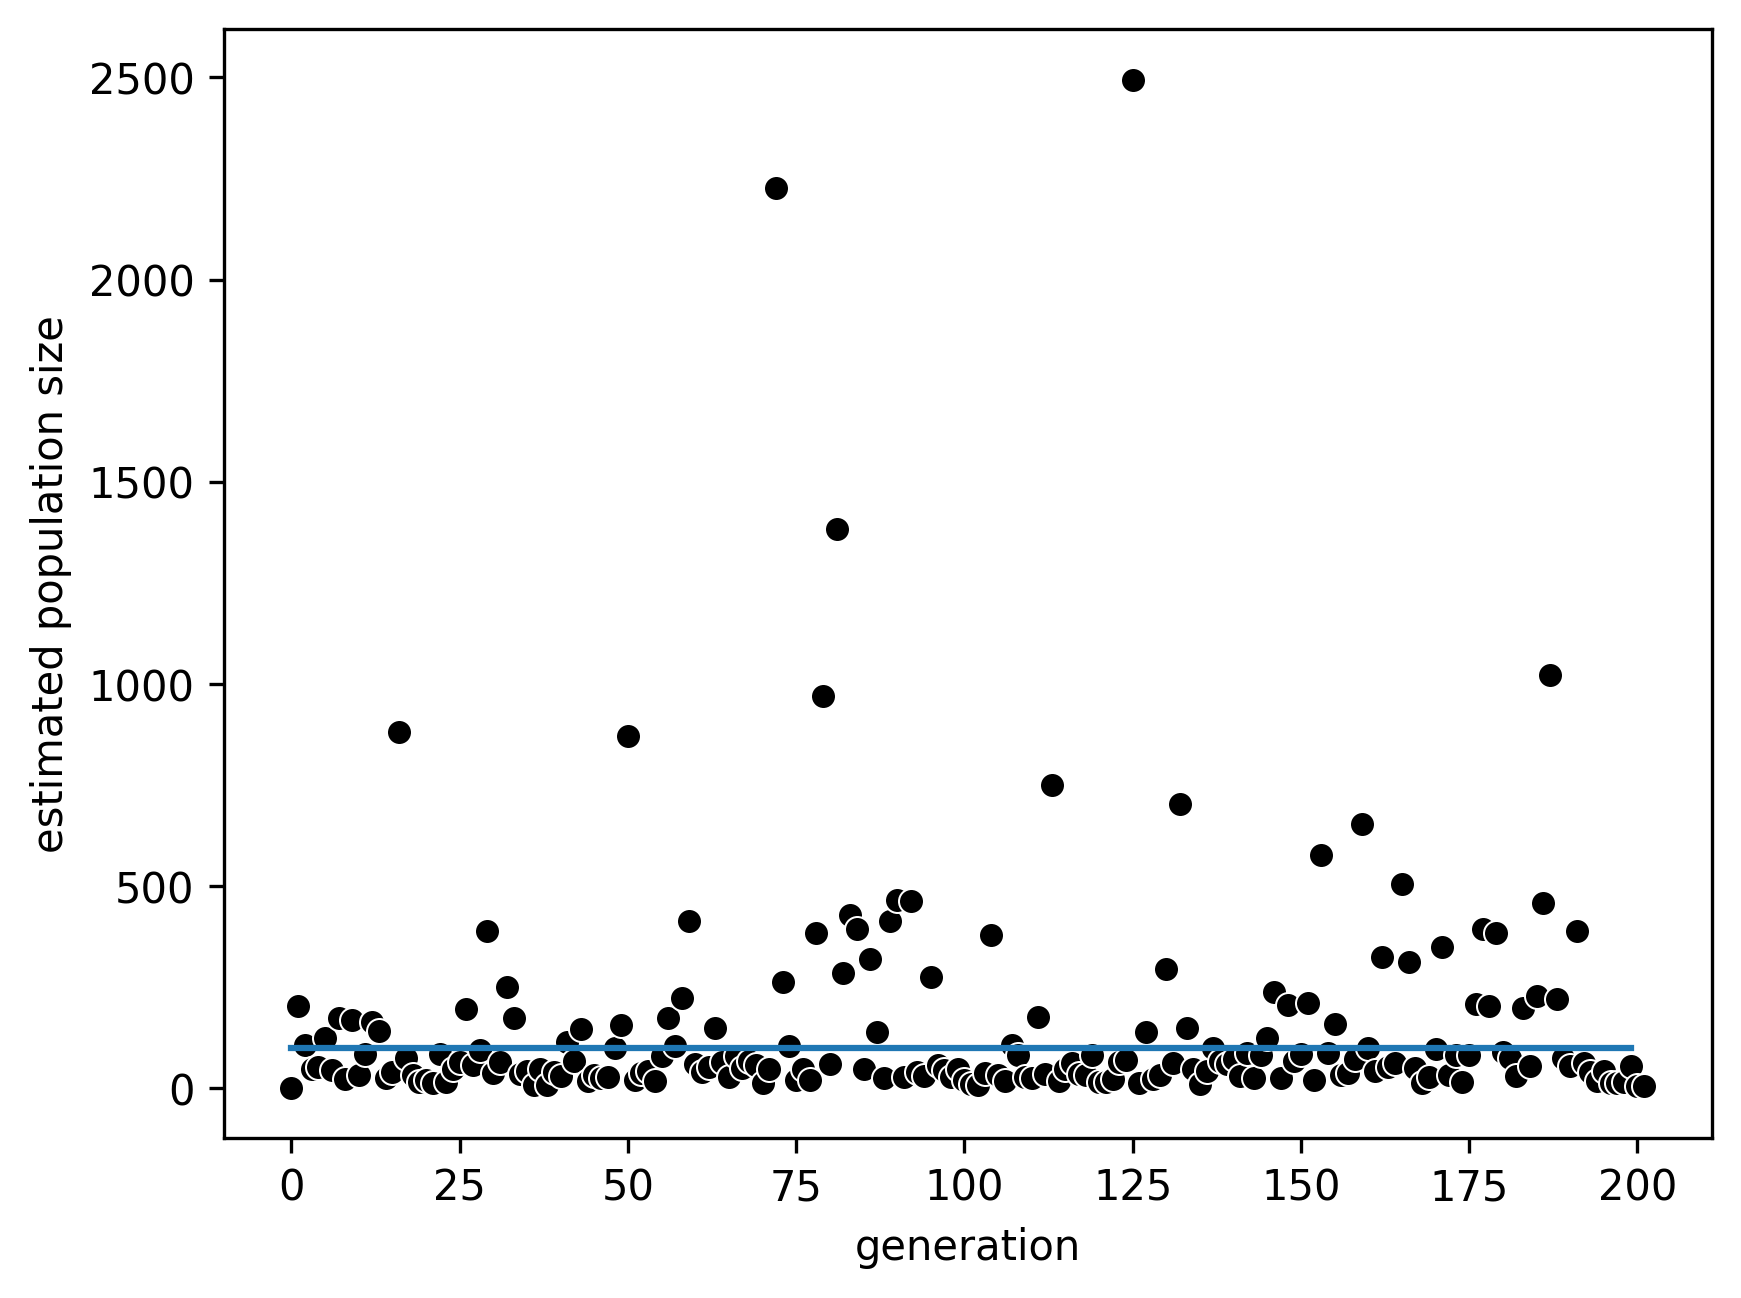
\includegraphics[height=0.25\textheight]{notebooks/notebooks/teeplots/notebook=ne-inference+replicate=0+treatment=control+viz=scatterplot-popsize-estimates+ext=}
  \end{minipage}%
  \begin{minipage}{.25\textwidth}
    \subcaption{Population Size Estimates}
    \label{fig:ne-process-example:singleton-est}
  \end{minipage}

  \vspace{0.25em}

  \begin{minipage}{.65\textwidth}
    \centering
    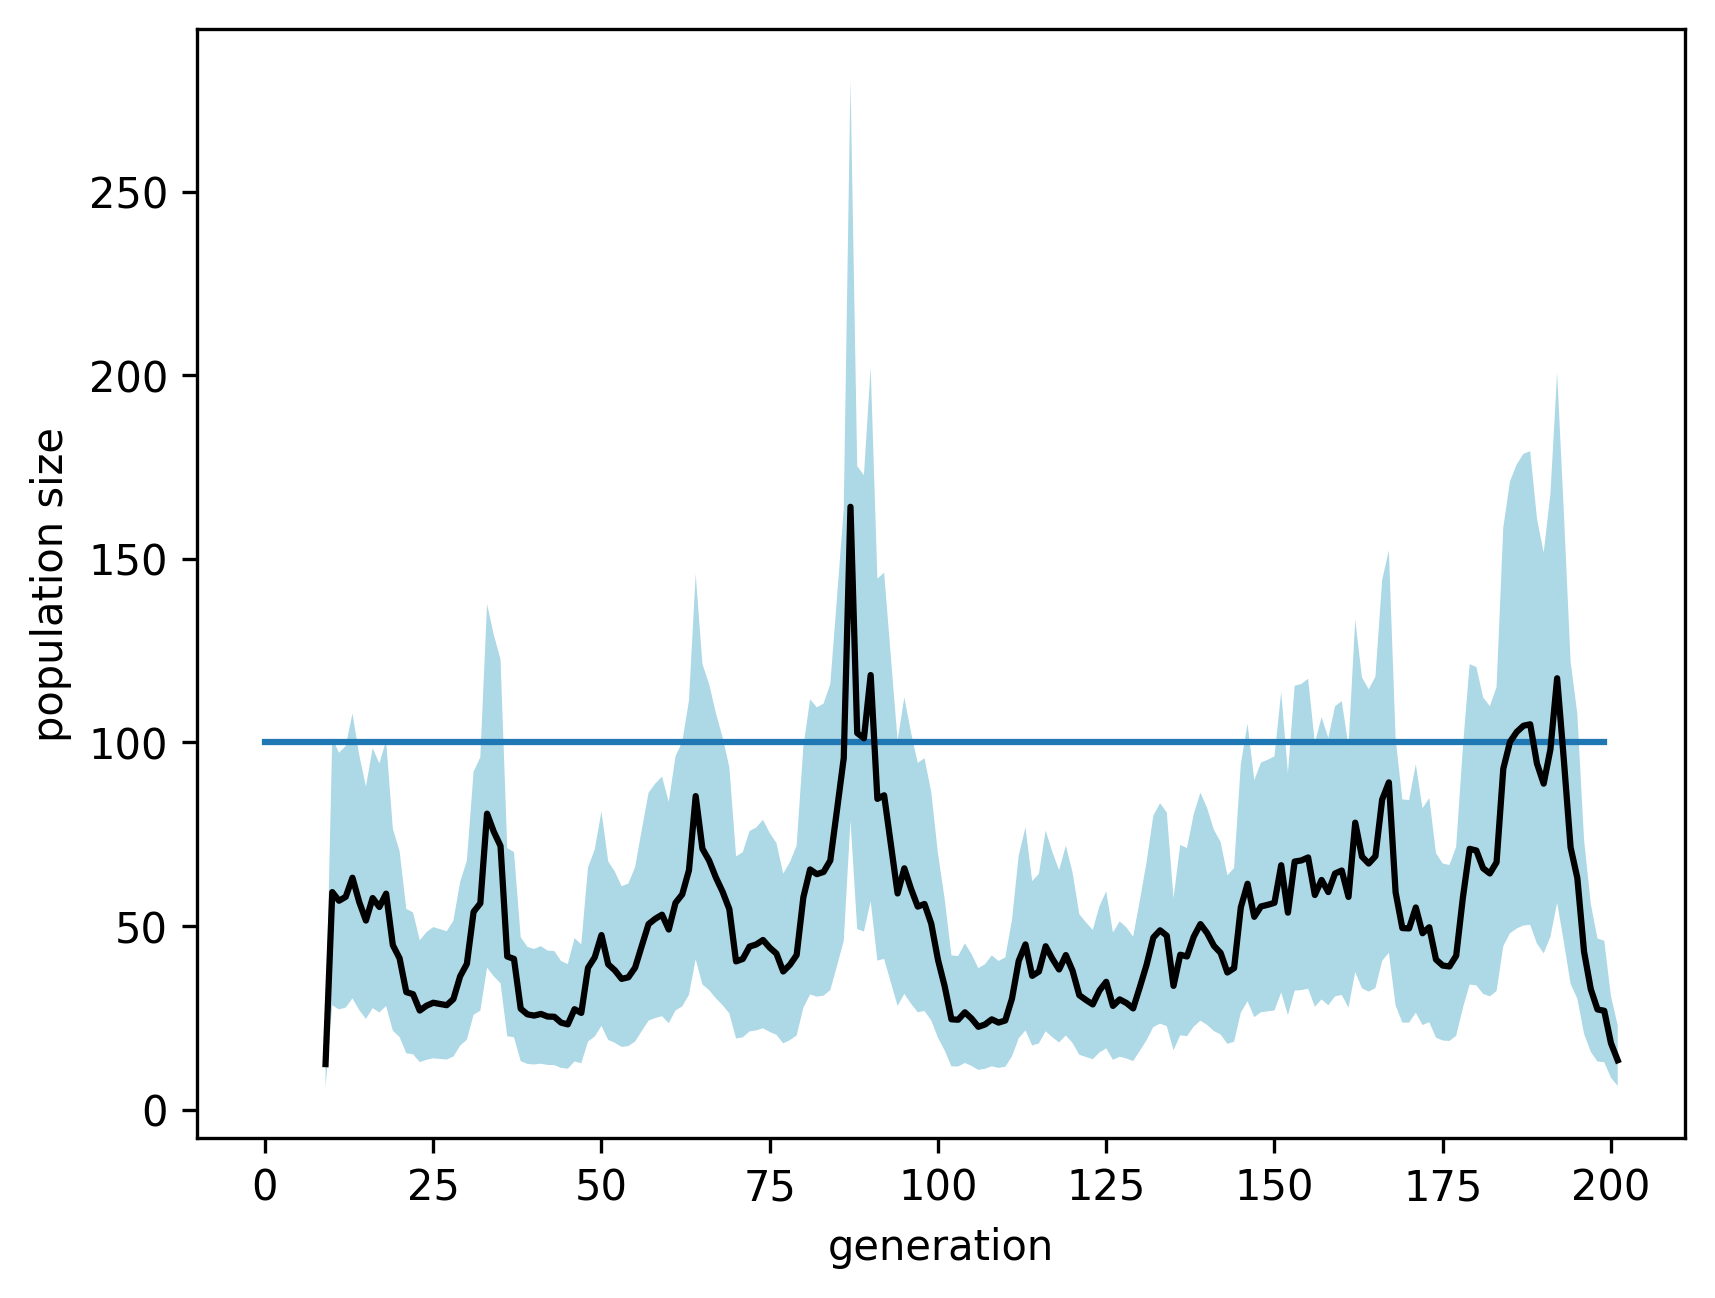
\includegraphics[height=0.25\textheight]{notebooks/notebooks/teeplots/notebook=ne-inference+replicate=0+treatment=control+viz=plot-running-estimation+x=rank+y=population-size+ext=}
  \end{minipage}%
  \begin{minipage}{.25\textwidth}
    \subcaption{Running Population Size Estimation with 95\% Confidence Intervals}
    \label{fig:ne-process-example:running-est}
  \end{minipage}

  \caption{
    Example population size estimation data.
    Differentia values are extracted from species-level annotation of a single extant population member (Subfigure \ref{fig:ne-process-example:differentia}).
    Subfigure \ref{fig:ne-process-example:singleton-est} shows one-off population size estimates at each generation from the corresponding differentia.
    To improve statistical informativeness, differentia values are grouped into a running pool of ten values to perform population size estimation.
    True population carrying capacity is annotated as a horizontal line.
    Note that systematic underestimation of ``carrying capacity'' population size is expected due to demographic factors excluding some population members from gene pool contributions.
    Figure \ref{fig:beta-explain} overviews the statistical mechanism used for population size distribution.
  }
  \label{fig:ne-process-example}
\end{figure}


% notebooks/notebooks/teeplots/notebook=ne-inference+replicate=0+treatment=control+viz=plot-running-estimation+x=rank+y=population-size+ext=.pdf
%
% notebooks/notebooks/teeplots/notebook=ne-inference+replicate=0+treatment=control+viz=scatterplot-differentia-magnitude+ext=.pdf
%
% notebooks/notebooks/teeplots/notebook=ne-inference+replicate=0+treatment=control+viz=scatterplot-popsize-estimates+ext=.pdf


% notebooks/notebooks/teeplots/notebook=ne-inference+replicate=0+treatment=bottleneck+viz=plot-running-estimation+x=rank+y=population-size+ext=.pdf
%
% notebooks/notebooks/teeplots/notebook=ne-inference+replicate=0+treatment=bottleneck+viz=scatterplot-differentia-magnitude+ext=.pdf
%
% notebooks/notebooks/teeplots/notebook=ne-inference+replicate=0+treatment=bottleneck+viz=scatterplot-popsize-estimates+ext=.pdf

% notebooks/notebooks/teeplots/notebook=ne-inference+replicate=0+treatment=range-expansion+viz=plot-running-estimation+x=rank+y=population-size+ext=.pdf
%
% notebooks/notebooks/teeplots/notebook=ne-inference+replicate=0+treatment=range-expansion+viz=scatterplot-differentia-magnitude+ext=.pdf
%
% notebooks/notebooks/teeplots/notebook=ne-inference+replicate=0+treatment=range-expansion+viz=scatterplot-differentia-magnitude+ext=.pdf
%
% notebooks/notebooks/teeplots/notebook=ne-inference+replicate=0+treatment=selection-pressure+viz=plot-running-estimation+x=rank+y=population-size+ext=.pdf
%
% notebooks/notebooks/teeplots/notebook=ne-inference+replicate=0+treatment=selection-pressure+viz=scatterplot-differentia-magnitude+ext=.pdf
%
% notebooks/notebooks/teeplots/notebook=ne-inference+replicate=0+treatment=selection-pressure+viz=scatterplot-popsize-estimates+ext=.pdf


Figure \ref{fig:ne-process-example} shows an example of population size inference over the course of an experiment.

Panel \ref{fig:ne-process-example:differentia} shows magnitudes of fixed differentia across the generational record extracted from a sample specimen at the end of the run.

Population size estimates can be computed at each generation using the maximum likelihood estimator (Equation \ref{eqn:popsize_mle}, as shown in Panel \ref{fig:ne-process-example:singleton-est}.
The true population size is annotated as a horizontal blue line.

To generate more robust inference, inference was pooled over rolling sets of 10 fixed differentia.
Population size estimates were again performed using Equation \ref{eqn:popsize_mle} with confidence interval bounds computed from Equations \ref{eqn:popsize_mle_ci_lb} and \ref{eqn:popsize_mle_ci_ub}.
Figure \ref{fig:ne-process-example:running-est} plots this running estimation.
Note that some discrepancy is expected between absolute population size (horizontal line) and effective population size $N_e$ (estimated) due to demographic factors.

\subsection{Population Size Inference Experiment}
\label{sec:population-size-inference-experiments}

The experiment tested the ability of the population size estimation process (Section \ref{sec:ne-process-example} to detect effective population size differences between populations and effective population size changes within a population over time.
Four different treatment conditions were compared: bottleneck, range expansion, selection pressure, and control.
Ten independent replicates were performed for each treatment.

The bottleneck treatment simulated a population reduction event.
The population size was kept at 100 for 67 generations, reduced an order of magnitude to 10 for 66 generations, and then returned to 100 for another 67 generations.

The range expansion treatment simulated gradual population size expansion.
The population size was initiated at at 10 for 67 generations, then increased linearly for 66 generations to 142 at generation 133, and then maintained at 142 for another 67 generations.

The selection-pressure treatment modified the selection intensity during the evolutionary process.
This reduced the effective population size by increasing the number of population members eliminated without contributing to the next generation. gene pool.
High selection pressure was applied for 67 generations (tournament size 8). Then, selection pressure was eliminated for 66 generations (tournament size of 1).
Finally, high selection pressure (tournament size 8) was reinstated for the last 67 generations.

The control treatment was run with a constant population size of 100 for 200 generations.

\subsection{Distributed Gene Prevalence Estimation}
\label{sec:dist-gene-prevalence-est}

\begin{sidewaysfigure}
  \centering
  \begin{minipage}{.7\textwidth} % adjust the width as needed

    \begin{minipage}{\textwidth}
      \centering
      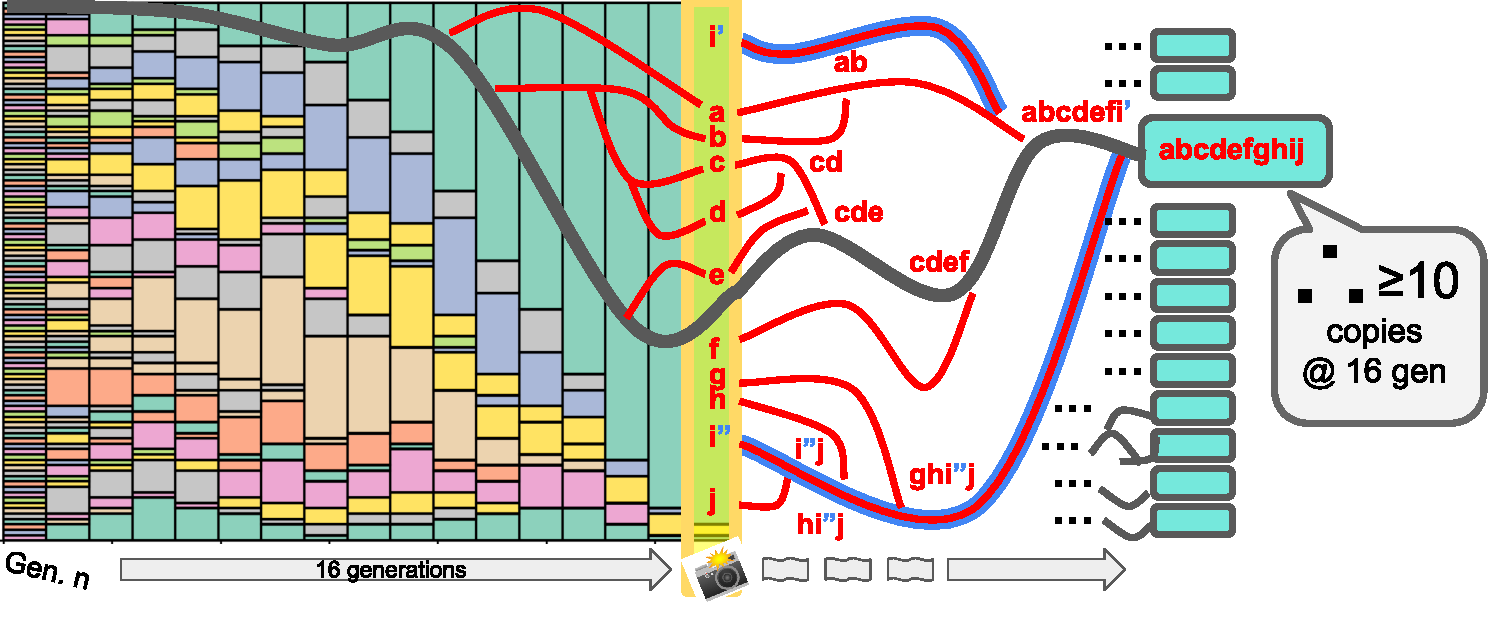
\includegraphics[height=0.30\textheight]{img/copy-count-snapshot}
      \subcaption{Cartoon depiction of delayed copy count estimation mechanism, annotated over Muller plot depicting weak selection over focal allele.
      }
      % \label{fig:ne-example-replicates:bottleneck}
    \end{minipage}%

    \vspace{1cm}

    \begin{minipage}{0.5\textwidth}
      \centering
      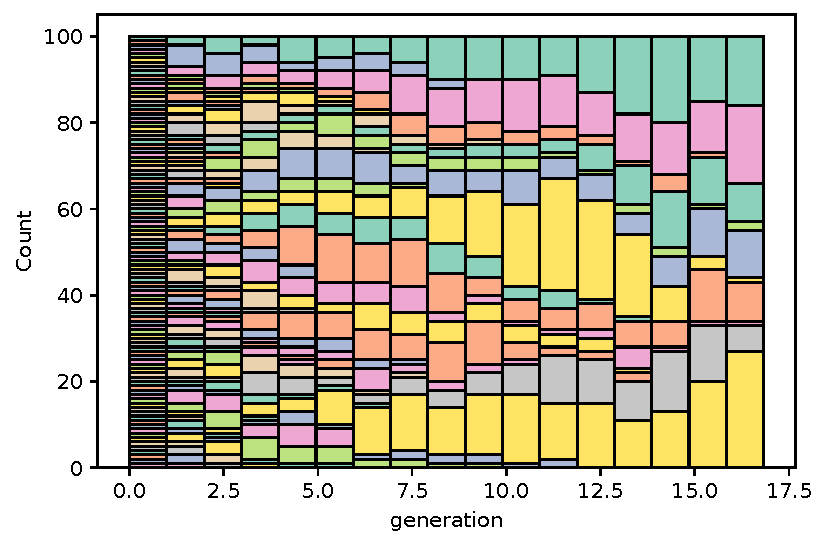
\includegraphics[height=0.2\textheight]{notebooks/notebooks/teeplots/fit=0.0+hue=clade+multiple=stack+ngen=16+npop=100+palette=set2+viz=histplot+x=generation+ext=}
      \subcaption{Muller plot depicting no selection for focal allele, ending with smaller copy count after 16 generations.}
      % \label{fig:ne-example-replicates:selection_pressure}
    \end{minipage}%
    \begin{minipage}{0.5\textwidth}
      \centering
      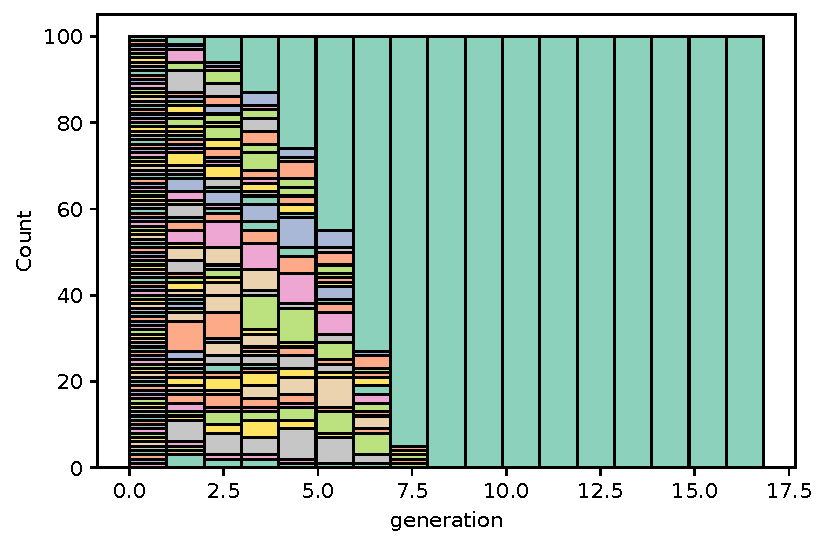
\includegraphics[height=0.2\textheight]{notebooks/notebooks/teeplots/fit=1.0+hue=clade+multiple=stack+ngen=16+npop=100+palette=set2+viz=histplot+x=generation+ext=}
      \subcaption{Muller plot depicting strong selection for focal allele, with fixation occuring before 16 generations.}
      % \label{fig:ne-example-replicates:control}
    \end{minipage}

  \end{minipage}
  \hfill % Creates horizontal space. Can also use \hspace{<len>}
  \begin{minipage}{.25\textwidth} % adjust the width as needed
    \caption{
      Proposed mechanism for detecting gene-level selection via a distributed delayed copy count estimation mechanism.
      Strata deposited at generation $n$ progress through 16 generations, with copy count of one allele growing due to selection.
      On the sixteenth generation, a ``snapshot'' is performed to set a random bit on field annotated onto each descendant differentia copy.
      In subsequent recombination events, set bits are exchanged between bit fields associated with common differentia.
      Copy count at generation $n + 16$ from can then estimated from these bit fields, with high copy count being suggestive of selection.
      Note that in this example collision between set bits $i'$ and $i"$ result in an undercount.
      This mechanism is associated with ``gene-level'' instrumentation (Figure \ref{fig:annotation-types}).
    }
    \label{fig:ne-example-replicates}
  \end{minipage}

\end{sidewaysfigure}


% notebooks/notebooks/teeplots/notebook=ne-inference+replicate=0+treatment=bottleneck+viz=plot-running-estimation+x=rank+y=population-size+ext=.pdf
%
% notebooks/notebooks/teeplots/notebook=ne-inference+replicate=0+treatment=control+viz=plot-running-estimation+x=rank+y=population-size+ext=.pdf
%
% notebooks/notebooks/teeplots/notebook=ne-inference+replicate=0+treatment=range-expansion+viz=plot-running-estimation+x=rank+y=population-size+ext=.pdf
%
% notebooks/notebooks/teeplots/notebook=ne-inference+replicate=0+treatment=selection-pressure+viz=plot-running-estimation+x=rank+y=population-size+ext=.pdf


Increases in allele prevalence tend to occur for alleles experiencing positive selection, but can also occur for selectively neutral alleles due to drift effects.
The key difference between the two is the \textit{rate} of increase within the population --- increases in prevalence due to drift tend to be slower than increases in prevalence due to selective effects, especially for large population sizes.

The proposed instrumentation mechanism uses gene-wise hereditary stratigraph instrumentation.
Selection is differentiated from drift dynamics by capturing an estimate of copy count of each gene's descendants after a fixed number of generations $g$ elapse.
If this copy count falls in the tails of the distribution expected after $g$ generations under a null hypothesis of pure drift dynamics, positive selection can be inferred.
Stronger positive selection will correlate with more extreme changes in copy count within the $g$ generation window.

In order to record estimated copy count, each ``fingerprint'' differentia within genes' hereditary stratigraph is bundled with an additional fixed-length, zero-initialized bit field annotation upon creation.
Each ``fingerprint'' has its own associated supplementary annotation.
This bit field is copied verbatim to descendants (i.e., gene copies passed to organismal offspring).

When the $g$th generation following a ``fingerprint'' differentia's creation elapses, a single bit is set at a random position of the supplementary annotation bit field.
During crossover, bit field annotations from the same generation with matching differentia are or'ed bitwise with each other.
In this manner, set bits gradually propagate among the records of all gene copies maintained in the population.

In this manner, annotations' bit counts converge to reflect the number of gene copies present after generational delay $g$.
Under count of gene copies is possible under this mechanism (due to positional collisions between set bits or gene copy extinctions immediately subsequent to generation $g$), but --- notably --- over count is not.
This conservative property supports confident detection of selection events --- these events would only be falsely detected due to true increases in copy count through drift, not due to instrumentation-associated error.
\footnote{This conservative property holds under the assumption of no spurious differentia collision.}
(This said, this conservative property could be sacrificed to increase sensitivity to larger copy counts with a given width bit field by only setting a bit at generation $g$ with small probability $p$.)

A bit field with of 8 bytes and a snapshot delay of 16 generations were arbitrarily chosen for experiments reported here.
Better sensitivity to weak selection events should be achievable through longer snapshot windows and larger bit fields, but likely this will be at the cost of diffusing signal from strong selection events.
Future work should seek a principled procedure to pick appropriate snapshot window length and bit field widths based on experimental objectives and properties of the underlying evolutionary system.

Positive selection can occur without advent of new allelic variants --- changes in environmental conditions can induce positive selection on an existing, potentially widespread allelic variant that was previously neutral.
This scenario is called a ``soft'' sweep \citep{hermisson2005soft}.
Weak sweeps should, in principle, be detectable to some extent through this methodology, as they involve increases in copy count at faster-than-drift rates.
However, weak sweeps on very-widespread alleles that quickly reach fixation will register only a weak signal on this instrumentation because increases in descendant copy count are spread across the large number of preexisting allele copies.
Although detectability of weak sweeps are not tested in this work, this consideration merits future work and may require alternate instrumentation designs.

\subsection{Positive Selection Inference Experiment}
\label{sec:positive-selection-inference-experiment}

A minimalistic experimental system was devised to test proposed methodology to detect positive selection on a novel allele.
We model the introduction of an atomic gene with tunable fitness advantage into an otherwise neutral background.

Each individual in the population was represented by a single floating-point number, representing a single focal gene.
Gene values were restricted between 0.0 and 1.0.
Fitness score was defined as the sum of its own value and a random number drawn from a continuous, uniform unit-valued distribution.
So, individuals' gene value corresponded directly to probabilistic fitness advantage.
For example, a value of 0.2 would give an average 20\% selective advantage.
Fitness scores for each individual were calculated once per generation and used for all tournaments.

All individuals were initialized with gene value 0.0.
At generation 50, one organism's gene value was set to either 0.0\footnote{The smallest representable positive value was set for fitness advantage treatment 0.0 so the introduced gene could be differentiated from the background gene. Infinitesimal small value was used so as to have no meaningfully detectable effect on selection.}, 0.1, or 1.0.
This operation was repeated at subsequent generations if the introduced gene value went extinct.
This procedure enabled comparison of a strong selective sweep for the gene (fitness advantage 1.0), a weaker selective sweep for the gene (fitness advantage 0.1) and a control treatment where no fitness advantage was introduced and pure drift dynamics were at play (fitness advantage 0.0).
Underlying selective sweep dynamics were measured by recording gene copy count at each generation.

Synchronous selection with tournament size 2 was performed each generation.
200 generations were simulated, with a constant population size of 400.
All parents for the upcoming population were selected before turnover of the entire population.
The crossover mating operator selected a gene value from among the two parents' genes with equal probability.
No mutation was applied.
Ten independent replicates were performed for each fitness advantage level treatment.

\subsection{Software \& Data}
\label{sec:software-data}

Software, data, and analyses used in this work are hosted on GitHub at \url{github.com/mmore500/hstrat-recomb-concept/tree/notebooks/notebooks}.

Data structures and algorithms associated with hereditary stratigraphy methodology are published in the hstrat Python package, made available on PyPi and on GitHub at \url{github.com/mmore500/hstrat} under the MIT license \citep{moreno2022hstrat}.
Recombination features developed for this project, as well as corresponding C++ implementations of hereditary stratigraphy data structures and algorithms, are on the project's near-term roadmap.

This project benefited greatly from open source scientific software, including BioPython \citep{cock2009biopython}, Distributed Evolutionary Algorithms in Python (DEAP) \citep{fortin2012deap}, Matplotlib \citep{hunter2007matplotlib}, NetworkX \citep{hagberg2008networkx}, Jupyter \citep{loizides2016jupyter}, pandas \citep{reback2020pandas,mckinney2010pandas}, SciPy \citep{pauli2020scipy}, seaborn \citep{waskom2021seaborn}, SymPy \citep{meurer2017sympy}, and tqdist \citep{sand2014tqdist}.
The Artificial Life data standard for phylogenies facilitated tool interoperation \citep{lalejini2019data}.
